\documentclass[aspectratio=169]{beamer}
%\documentclass{beamer}
\usepackage{graphicx,amsmath}
\usepackage{listings}
\usepackage{algorithmicx}
\usepackage{algorithm}
\usepackage{algpseudocode}
\usepackage{microtype}
\usepackage{tikz}
\usepackage{wrapfig}
\usepackage{bm}
\usepackage{soul}
\usepackage{subcaption}
\renewcommand{\vec}{\mathbf}
\usepackage{xcolor}
\renewcommand{\Re}{{\rm I\!R}}

\author[Maarten de Waard]{Maarten de Waard\\\small{Supervised by Diederik
	Roijers and Sander Bakkes}}
	\title[O-MCTS for GVGP]{Monte Carlo Tree Search with Options\\for General Video Game Playing}
\date{February 22\textsuperscript{nd}\\Public Thesis Defense}
\usetheme{Berkeley}

\begin{document}
\setbeamertemplate{blocks}[rounded][shadow=true]
\begin{frame}
	\vspace{-4.7em}
	\centerline{
	\includegraphics[scale=.8]{includes/LogoUvA}
	}
	%\hspace{1cm}
	%\vspace{-1cm}
	\maketitle
\end{frame}

\section{Introduction}

\begin{frame}
	\frametitle{Contents}
	\tableofcontents
\end{frame}

\begin{frame}
	\frametitle{Introduction}
	\begin{block}{General Video Game Playing}
		\begin{itemize}
			\item Games as problem setting
			\item Real world problems can be modelled as games
		\end{itemize}
	\end{block}
	\begin{block}{Artificial Intelligence}
		\begin{itemize}
			\item A general AI algorithm is capable of solving different problems
			\item Creating general AI algorithms is considered a step towards \emph{strong AI}
		\end{itemize}
	\end{block}
\end{frame}

\section{Background}

\subsection{General Video Game Playing}
\begin{frame}
	\frametitle{General Video Game Playing \cite{perez2014, schaul2013video}}
	\begin{block}{General Video Game AI competition}
		\begin{itemize}
			\item Several sets of games
			\item Compare algorithms by testing them on many games
			% Move this to first slide of experiments
			% \item Framework:
			% 	\begin{itemize}
			% 		\item 40 ms of action time
			% 		\item Forward model as simulator
			% 	\end{itemize}
		\end{itemize}
	\end{block}
	\begin{block}{Video Game Description Language}
		\begin{itemize}
			\item Aims to be a clear, human readable and unambiguous
				description language for games
			\item Define a game with two files
		\end{itemize}
	\end{block}
\end{frame}

\subsection{Markov Decision Processes}
\begin{frame}
	%TODO: Is dit de juiste cite?
	\frametitle{Markov Decision Processes (MDPs) \cite{sutton1998reinforcement}}
	States, actions, transitions, reward. Maximize cumulative reward over time.
	\begin{figure}
	\centering
	\includegraphics[height=.6\textheight]{includes/mdp}
	\end{figure}
\end{frame}
\begin{frame}
	\frametitle{Games as MDPs}
	\begin{figure}
	\centering
	\includegraphics[height=.9\textheight]{includes/gameboy}
	\end{figure}
\end{frame}

\subsection{Monte Carlo Tree Search}
\begin{frame}
	\frametitle{Monte Carlo Tree Search\cite{gelly2006modification}}
	\begin{figure}
	\centering
	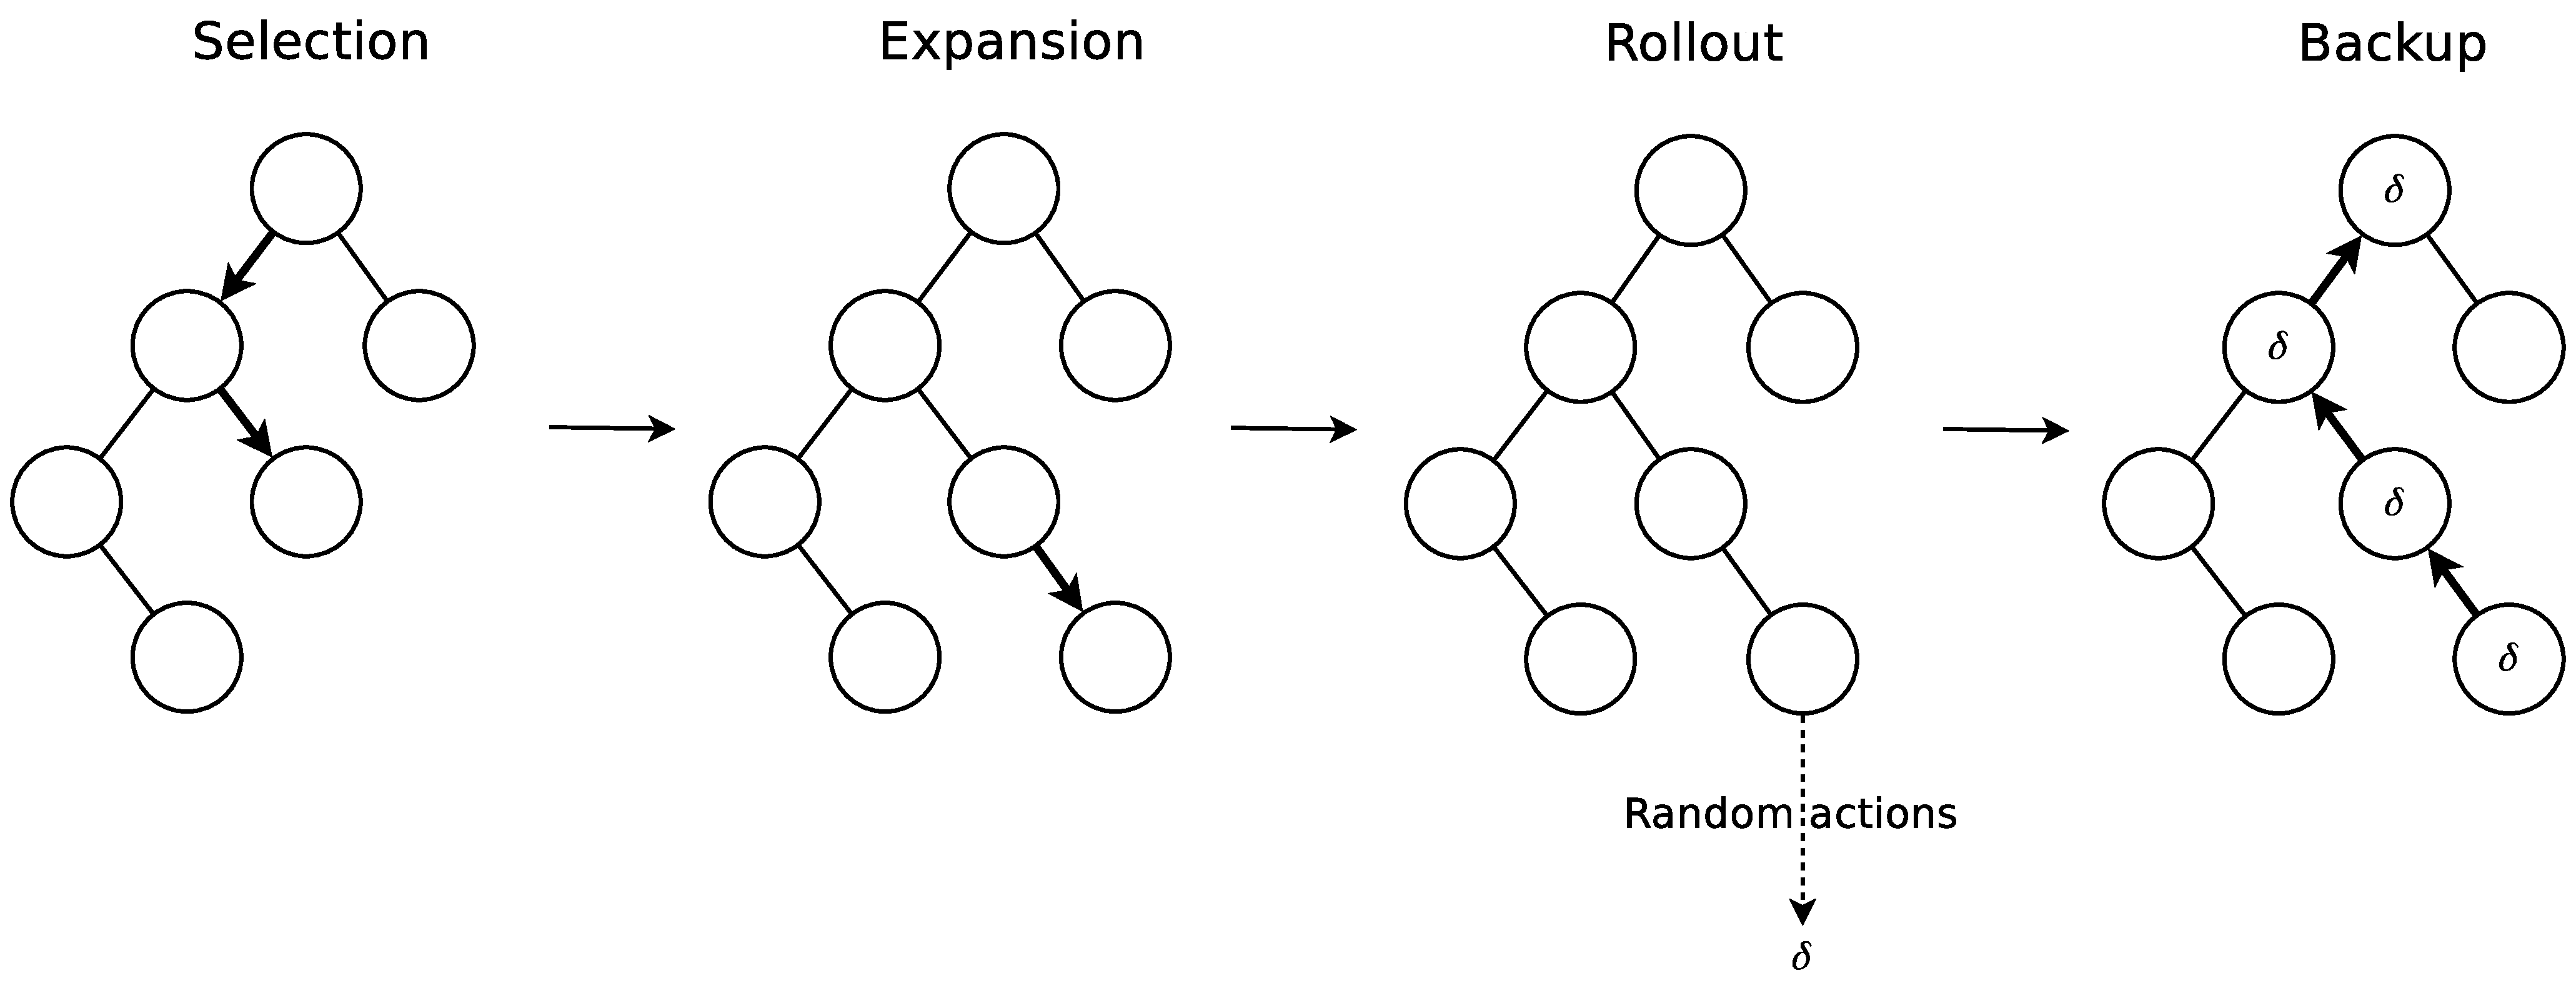
\includegraphics[width=.94\textwidth]{includes/mcts-wide}
	\end{figure}
\end{frame}

\subsection{Options}
\begin{frame}
	\frametitle{Options \cite{sutton1999between, barto2003recent}}
	\only<1-2>{
		\begin{itemize}
			\item Sequence of actions for reaching a specific subgoal
			\visible<2>{\item For example: ``move towards the nearest NPC''}
		\end{itemize}
		\visible<2>{
			\begin{figure}
				\centering
				\includegraphics[height=.6\textheight]{includes/goToMovableOption}
			\end{figure}
		}
	}
	\only<3-4>{
		\begin{block}{Formally, $\langle I, \pi, \beta \rangle$}
			\begin{itemize}
				\item $I = $ initiation set \onslide<4>{-- any state with NPCs in it}
				\item $\pi = $ policy \onslide<4>{-- the arrows in the previous slide}
				\item $\beta = $ termination condition \onslide<4>{-- the monster's location = the avatar's location}
			\end{itemize}
		\end{block}
	}
\end{frame}

\subsection{SMDP Q-learning}
\begin{frame}
	\frametitle{SMDP Q-learning \cite{sutton1999between}}
	\begin{block}{Q-learning}
		\begin{itemize}
			\item Q-learning is a simple reinforcement learning algorithm
			%TODO: Dit kan beter
			\item Saves a combination of the current reward and the best
				possible future reward
		\end{itemize}
	\end{block}
	\begin{block}{SMDP Q-learning}
		\begin{itemize}
			\item Version for Semi-MDPs: actions have variable time length
			\item Proposed in combination with options
		\end{itemize}
	\end{block}
\end{frame}

\section{General Video Game Playing}
\begin{frame}
	\frametitle{Framework}
	\begin{columns}
		\column{.55\textwidth}
		\begin{block}{Terminology}
			\begin{itemize}
				\item Games with levels
				\item Sprites
				\item Avatar
				\item NPC
				\item Movable vs. Non-movable
			\end{itemize}
		\end{block}
		\begin{block}{GVGAI}
			\begin{itemize}
				\item Forward model as simulator
				\item 40 milliseconds action time
				\item 1 second initialization time
			\end{itemize}
		\end{block}
		\column{.4\textwidth}
			\includegraphics[width=\columnwidth]{includes/zelda}
	\end{columns}

\end{frame}
\begin{frame}[fragile, allowframebreaks]
	\frametitle{Game Description}
	\begin{lstlisting}[caption=Game Description, frame=tb]
BasicGame
  SpriteSet
    movable >
      avatar    > MovingAvatar img=avatar
      prey      > img=monster
        inactivePrey    > RandomNPC cooldown=3000
        slowPrey        > RandomNPC cooldown=10
        fastPrey        > RandomNPC cooldown=2




  LevelMapping
    A   > avatar
    I   > inactivePrey
    S   > slowPrey
    F   > fastPrey

  InteractionSet
    prey avatar     > killSprite scoreChange=1
    movable wall    > stepBack

  TerminationSet
    SpriteCounter stype=prey limit=0 win=True
    Timeout limit=100 win=False
	\end{lstlisting}
\end{frame}

\begin{frame}[fragile]
	\frametitle{Level Description}
	\begin{columns}[c]
		\column{.5\textwidth}
		\centering
		\begin{lstlisting}[caption=Level, frame=tb, xleftmargin=.3\textwidth, xrightmargin=.3\textwidth]
wwwwwww
wA    w
w     w
w     w
w    Iw
wwwwwww
		\end{lstlisting}
		\column{.5\textwidth}
		\includegraphics[width=\columnwidth]{includes/prey}
	\end{columns}
\end{frame}

\begin{frame}
	\frametitle{Option Set}
	\begin{itemize}
		\item Action
		\item Avoid nearest NPC
		\item Go near movable
		\item Go to movable
		\item Go to nearest sprite of type
		\item Go to position
		\item Wait and shoot
	\end{itemize}
\end{frame}

\section{O-MCTS}
\begin{frame}
	\frametitle{Option MCTS}
	\begin{columns}
		\column{.6\textwidth}
		\small
		\vspace{-.5em}
		\begin{algorithmic}[1]
			\While {time\_taken $<$ max\_time}
				\State $s \gets $ current state
				\While {stopping condition not met}
					\If{not all options expanded}
						\State $\omega \gets$ unexplored option
						\State $a \gets \mathsf{get\_action}(\omega, s)$ 
						\State $s' \gets \mathsf{expand}(s, a)$ 
						\State \textbf{break} \label{alg:omcts:break}
					\Else \label{alg:omcts:sexpand}
						\State $s \gets$ child node from \emph{selection}
					\EndIf \label{alg:omcts:eexpand}
				\EndWhile
				\State $\delta \gets \mathsf{rollout}(s', \omega)$
				\State $\mathsf{back\_up}(s', \delta)$
			\EndWhile
			\State \Return {action from option with highest value}
		\end{algorithmic}

		\column{.4\textwidth}
		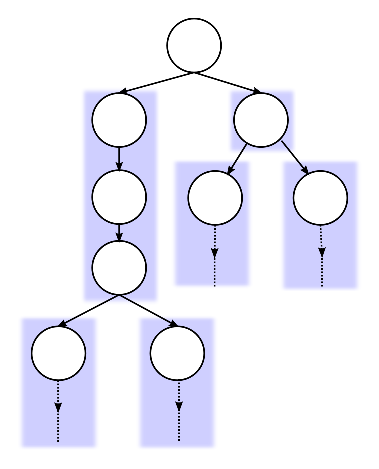
\includegraphics[width=\columnwidth]{includes/omcts}
	\end{columns}
\end{frame}

\section{OL-MCTS}
\begin{frame}
	\frametitle{Option Learning MCTS - Option Values}
	\begin{block}{Option Types}
		\begin{itemize}
			\item Type: \emph{go to movable}, \emph{avoid nearest NPC}, etc.
			\item Subtype: one subtype for each type of sprite
				\begin{itemize}
					\item The \emph{go to movable option} in \textit{zelda} has
						one subtype for the monsters and one for the key
				\end{itemize}
			\item The \emph{action option} has a subtype for each action
		\end{itemize}
	\end{block}
	\begin{block}{Option Values}
		\begin{itemize}
			\item Use mean and variance of option's expected return:
			\item $r_o = r_{t} + \gamma r_{t+1} + \gamma^2 r_{t+2} + \ldots + \gamma^n r_{t+n}$
			\item Save this value for each option \emph{subtype} after the option is finished
		\end{itemize}
	\end{block}
\end{frame}
\begin{frame}
	\frametitle{Option Learning MCTS - Crazy Stone Algorithm \cite{coulom2007efficient}}
	\begin{columns}
		\column{.5\textwidth}
			\begin{itemize}
				\item Formula to bias towards selecting child node for option
					with higher value or variance
				\item Usable for both the \emph{exploration} and
					\emph{selection} step in the first $v$ node visits
			\end{itemize}
		\column{.5\textwidth}
			\centering
			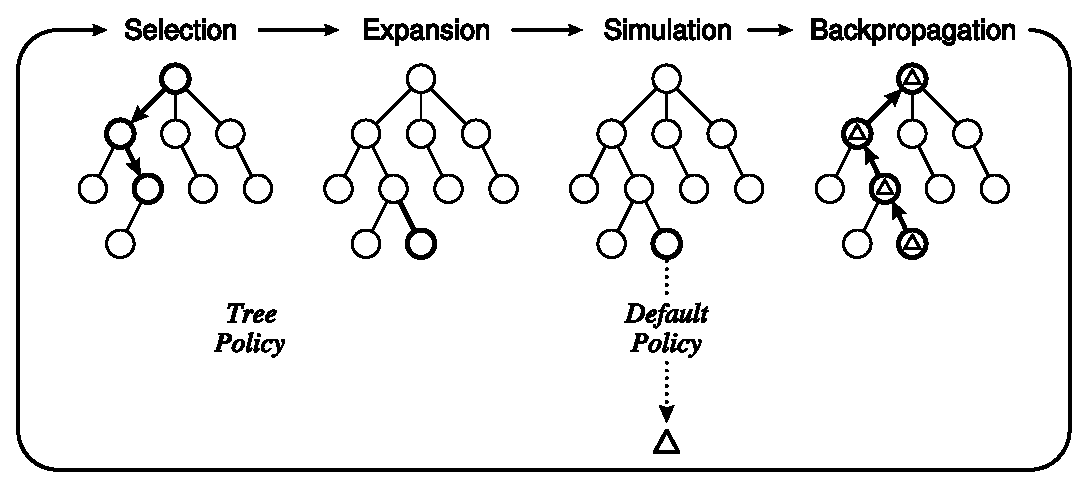
\includegraphics[height=.94\textheight]{includes/mcts}
	\end{columns}
\end{frame}

\section{Experiments}
\begin{frame}
	\frametitle{SMDP Q-learning vs. MCTS}
	\begin{figure}
	\centering
	\makebox[\columnwidth]{\includegraphics[width=1.05\textwidth]{includes/qLearningWins}}
	\end{figure}
	\begin{figure}
	\centering
	\makebox[\columnwidth]{\includegraphics[width=1.05\textwidth]{includes/qLearningScores}}
	\end{figure}
\end{frame}

\begin{frame}
	\frametitle{O-MCTS vs. MCTS}
	\begin{figure}
	\centering
	\makebox[\columnwidth]{\includegraphics[width=1.05\textwidth]{includes/wins}}
	\end{figure}
	\begin{figure}
	\centering
	\makebox[\columnwidth]{\includegraphics[width=1.05\textwidth]{includes/scores}}
	\end{figure}
\end{frame}

\begin{frame}
	\frametitle{OL-MCTS vs. O-MCTS}
	\begin{figure}
	\centering
	\makebox[\columnwidth]{\includegraphics[width=1.05\textwidth]{includes/winsOLMCTS}}
	\end{figure}
	\begin{figure}
	\centering
	\makebox[\columnwidth]{\includegraphics[width=1.05\textwidth]{includes/scoresOLMCTS}}
	\end{figure}
\end{frame}

\begin{frame}
	\frametitle{Totals}
	\begin{figure}
	\centering
	\includegraphics[height=.6\textheight]{includes/totalsThesis}
	\end{figure}
\end{frame}

\section{Demo}
\begin{frame}
	\frametitle{Demo}
\end{frame}

\section{Conclusion}
\begin{frame}
	\frametitle{O-MCTS}
	\begin{columns}
		\column{.3\textwidth}
		\begin{block}{Outperforms MCTS in}
			\begin{itemize}
				\item \textit{missile command}
				\item \textit{bait}
				\item \textit{camel race}
				\item \textit{survive zombies}
				\item \textit{firestorms}
				\item \textit{lemmings}
				\item \textit{fire caster}
				\item \textit{overload}
				\item \textit{zelda}
				\item \textit{chase}
			\end{itemize}
		\end{block}
		\column{.6\textwidth}
		The new algorithm \ldots
			\begin{itemize}
				\item outperforms SMDP Q-learning on every game 
				\item excels in games with small level grid, low number of
					sprites and high complexity
				\item look further ahead than most tree searching alternatives
				\item performs below expectation on games with many sprites or a
					big level grid
			\end{itemize}
	\end{columns}
\end{frame}

\begin{frame}
	\frametitle{OL-MCTS}
	The learning variant, OL-MCTS \ldots
	\begin{itemize}
		\item is shown to learn for the games \textit{prey} and \textit{bait}
		\item this indicates it is possible to improve O-MCTS with learning
		\item needs more work
	\end{itemize}
\end{frame}

\begin{frame}
	\frametitle{Future Work}
	\begin{block}{O-MCTS}
		\begin{itemize}
			\item Improve option set. Find out which options are useful, try
				faster methods than A Star
			\item Multi-objective version, to balance time cost, score and
				winning
		\end{itemize}
	\end{block}
	\begin{block}{OL-MCTS}
		\begin{itemize}
			\item Remove infeasible options from the option set entirely
			\item Try other backup methods
		\end{itemize}
	\end{block}
\end{frame}

\section{References}
\begin{frame}%[allowframebreaks]
	\frametitle{References}
	\tiny{\bibliographystyle{abbrv} }
	\bibliography{bib}
\end{frame}

\end{document}
